\chapter{Implementation}
\label{chapter:implementation}

The architecture of the application contains two main modules: the user interface (UI) in the form of a Web Application, presented in \autoref{sec:impl-wa} and the actual implementation of the conversational agent, detailed in \autoref{sec:impl-conversational-agent}.

In the next sections reference to the chat client, chat server and chat-bot signify the front end user interface, the back end of the web application and the conversational agent program respectively.

\section{Web Application}
\label{sec:impl-wa}

The web application is the interface with the help of which the user interacts with the conversational agent. It implements a chat client, a program where the user can input its questions and see the answers processed by the conversational agent and returned by the chat server. It also implements a chat server that connects to the chat-bot's endpoint. After the connection succeeds, the chat server passes the query received from the client to the chat-bot, waits for a reply and then sends the reply back to the client.

The chat client is described in \autoref{sub-sec:impl-wa-front-end} and the chat server is described in \autoref{sub-sec:impl-wa-back-end}. The chat-bot's endpoint of the aforementioned connection between him and the chat server is explained at length in \autoref{sec:impl-conversational-agent}.

\subsection{Front End}
\label{sub-sec:impl-wa-front-end}

The front end is written in HTML, CSS and JavaScript and it is composed of two main screens: the first page where the user can input the name of the personality he wishes to speak to; the second page, the actual chat box, where the conversation is displayed, and the input box, where the user can write the question and submit it.

The first screen is shown in \autoref{fig:web-app-first}. Clicking the {\em Enter} button would send a request to the chat server that would later on initialize the chat-bot with the inputted personality.

\begin{figure}[htb]
  \centering
  \captionsetup{justification=centering}
  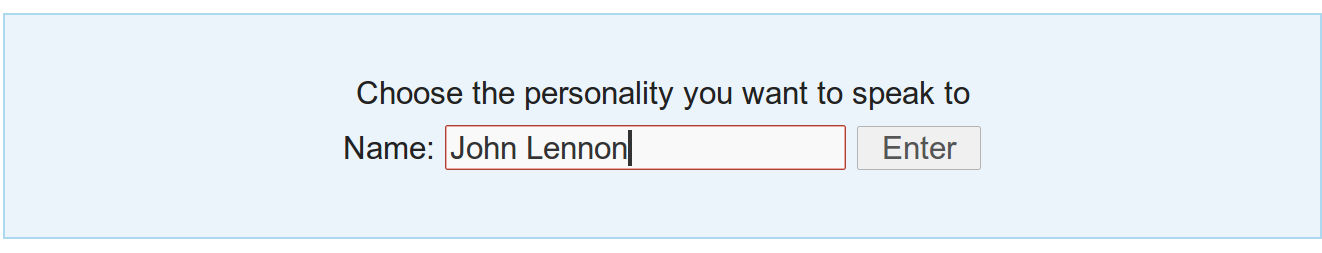
\includegraphics[width=\textwidth]{src/img/web-app-first.png}
  \caption[Web Application - First Window]{The first page of the Web App where the user can input the name of the personality he wants to talk with}
  \label{fig:web-app-first}
\end{figure}

In \autoref{fig:web-app-second}, the chat box containing a few questions and answers can be seen. At the bottom of the chat box there is the input text box where the user can write its questions and submit them.

\begin{figure}[htb]
  \centering
  \captionsetup{justification=centering}
  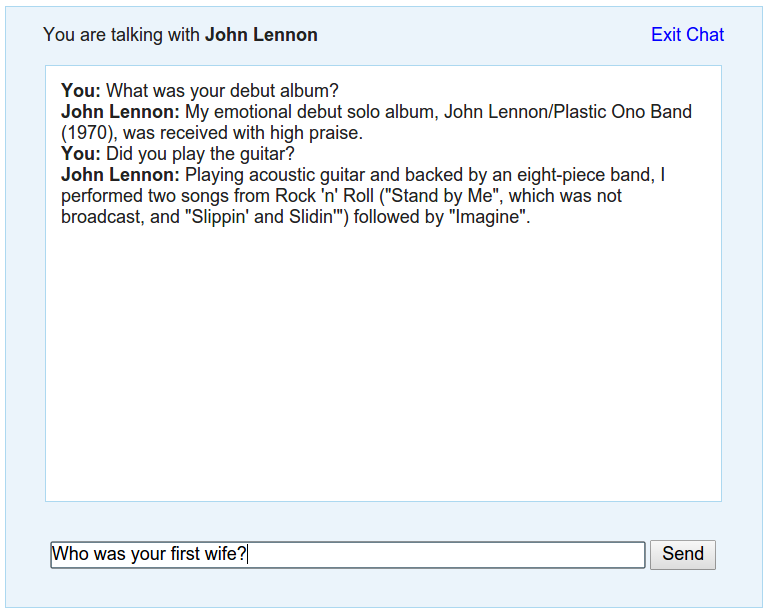
\includegraphics[width=\textwidth]{src/img/web-app-second.png}
  \caption[Web Application - Second Window]{The page where the user can submit questions and see the replies}
  \label{fig:web-app-second}
\end{figure}

The conversation is saved on the client-side, in memory, using JavaScript, and is persistent until the page is refreshed or closed.

The questions are submitted by sending a synchronous HTTP GET request to the server. The request contains the question. The request is sent using AJAX (Asynchronous JavaScript + XML) and contains a random generated number in the URL so that the browser doesn't serve a cached page. For example, \url{http://<hostname>/chatbot.php?question=What+was+your+debut+album\%3F\&t=0.023473239736631513} sends the question {\em "What was your debut album?"} to the chat server.

\subsection{Back End}
\label{sub-sec:impl-wa-back-end}

The server side of the web application is made up of XAMPP\footnote{\href{https://www.apachefriends.org/index.html}{XAMPP Website}\url{https://www.apachefriends.org/index.html}}\textsuperscript{,}\footnote{XAMPP is a bundle containing the Apache HTTP server, a MySQL server and a PHP and Perl interpreter} and the PHP scripts that implement the connection with the chat-bot.

Functionally, the communication is accomplished by using a local socket to socket connection between the web server and the conversational agent server. A snippet of the code the shows the principles of communication between the two servers is presented in \autoref{lst:backend}. The main aspects of the program are highlighted through comments in the code. The flow of the communication is shown in \autoref{fig:client-server-flow}.

\lstinputlisting[language=PHP, firstline=11, lastline=32, caption=Socket communication between the web server and the chat-bot, label=lst:backend]{src/code/chatbot.php}

\begin{figure}[htb]
  \centering
  \captionsetup{justification=centering}
  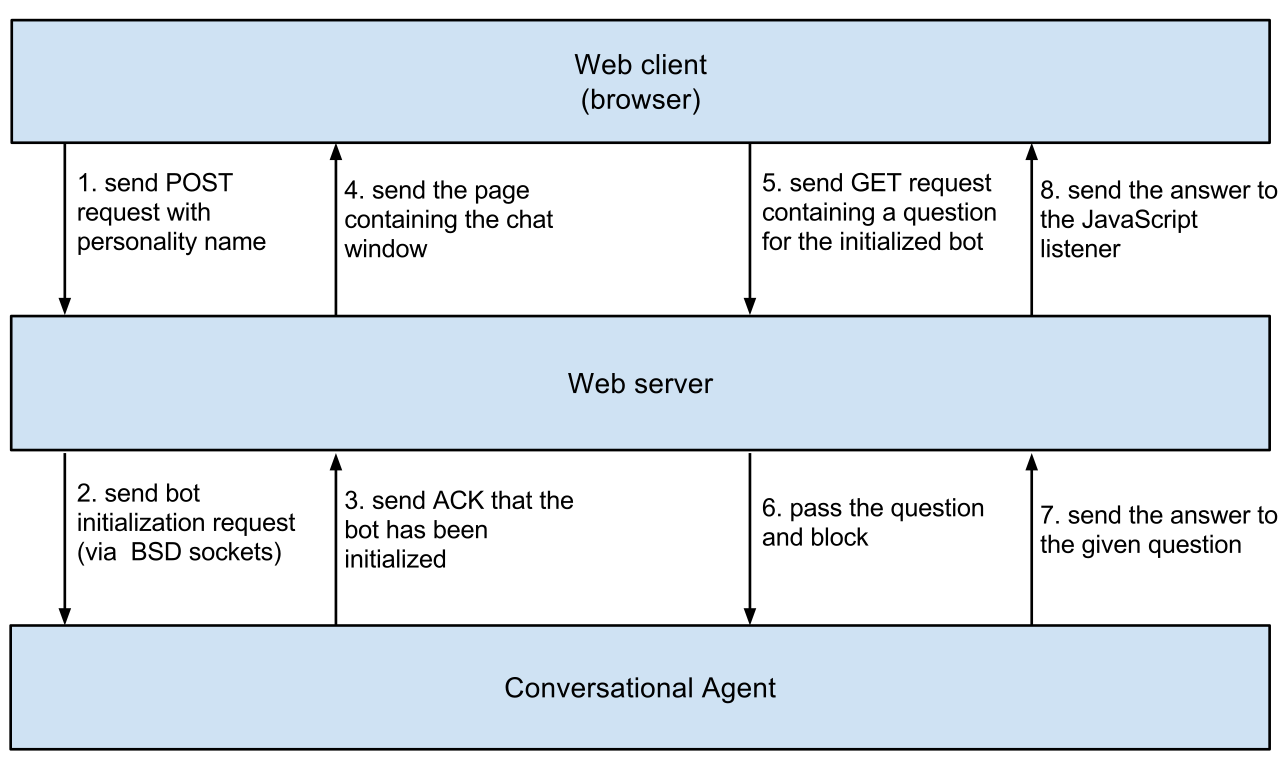
\includegraphics[width=\textwidth]{src/img/client-server-flow.png}
  \caption[Order of requests between client and servers]{The communication flow between the client, web server and conversational agent server}
  \label{fig:client-server-flow}
\end{figure}



\section{Conversational Agent}
\label{sec:impl-conversational-agent}

This section contains the architectural decisions and the implementation details of the conversational agent. First, in \autoref{sub-sec:impl-ca-rule-based}, the  rule-based system approach using the DBpedia ontology and the ChatScript engine is described in short. Next, the approach to implementation employing the {\em answer sentence selection} method is presented at length.

\subsection{Rule-based System Approach}
\label{sub-sec:impl-ca-rule-based}

This approach relies on the chat-bot engine ChatScript (see \autoref{sec:chatscript}) and its scripting language. For the chat-bot to answer question, it must match them against the rules in the ChatScript files. Because multiple personalities can be instantiated and no two people share the same biography, it is imperative that a set of ChatScript files containing rules must be generated for each personality the user wants to talk to.

To generate the pattern inside a ChatScript rule and also the relevant response to a certain pattern, a solution is needed for expressing different properties and for finding their value in a Wikipedia article respectively. These two methods are described in the next couple of sections.

\subsubsection{Expressing a Property}

Expressing a property implies finding a statistical model that maps properties extracted from DBpedia to a set of word groups that appear in Wikipedia and that relate to the value of said property. In order to find the best way a property is expressed, a large number of properties from a lot of DBpedia pages are needed. After filtering out properties that are not necessary for building the conversational agent, the only task remaining is to parse the Wikipedia corpus to find the value of that property in the sentences where the person which each article is about appears in \cite{Bogatu}.

The best way to identify the way a property might be expressed is to analyze the parse tree generated using Stanford CoreNLP and observe how the value of a property influences the structure (topology) of this parse tree. After interpreting numerous examples of sentences that include the value of a property and theorizing the way a property might be expressed, the conclusion is that a good way to express a property is using the words on the path from the property (excluding the value) to the root verb.

Having the desired sentence identified, we annotated it using Stanford CoreNLP and obtained a syntactic parse tree.  Analyzing this tree, we determined that the root is the verb directly connected with the subject. Having the parse tree, we considered that the best way to express the property is the path from that property to the root verb.

Some examples of entries in the knowledge base are presented in \autoref{table:express-property}. The property is extracted from DBpedia and the lexicalization represents an enumeration of ways the given property appears to be expressed in the Wikipedia articles.

\begin{table}[htb]
  \centering
  \begin{tabular}{r|l}
    \textbf{DBpedia Property} & \textbf{Lexicalizations} \\
    \hline
    birthDate & born, born in \\
    almaMater & receive in, graduate as \\
    award & award, receive \\
    college & graduate from, attend \\
    deathPlace & die in \\ 
    profession & serve in, become \\
    spouse & marry, marry to \\
  \end{tabular}
  \caption{Examples of how specific DBpedia properties are most often expressed}
  \label{table:express-property}
\end{table}

Two examples of syntactic parse trees can be seen in \autoref{fig:parse-trees}. The parse tree in \autoref{fig:parse-tree1} is for the sentence "Albert Einstein was born in Ulm." It can be noticed that the DBpedia property that connects "Albert Einstein" and "Ulm" and for which we want to identify a
lexicalization is the "birthPlace" property and the lexicalization is "born in". In the second example, \autoref{fig:parse-tree2}, the method still stands, and having the "award" property and the "Nobel Prize" associated value, it can be determined that the manner of expressing this property is with the "receive" lexicalization.

\begin{figure}[htb]
\begin{minipage}{.5\textwidth}
  \centering
  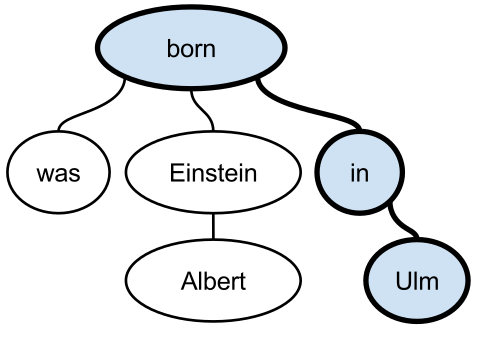
\includegraphics[width=\textwidth]{src/img/parse-tree2.png}
  \caption[Parse tree with path expressing a property, Example 1]{Parse tree for "Albert Einstein was born in Ulm." with path expressing a DBpedia property being highlighted}
  \label{fig:parse-tree1}
\end{minipage}
\begin{minipage}{.5\textwidth}
  \centering
  \captionsetup{justification=centering}
  \centering
  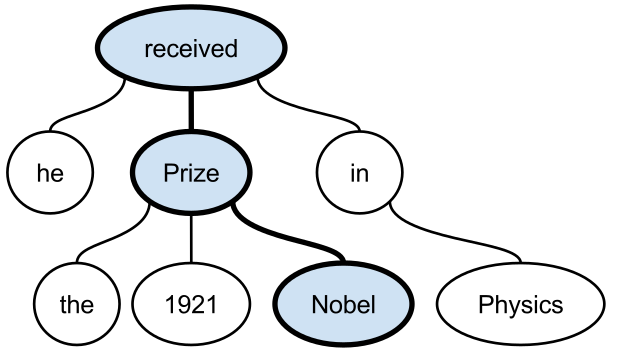
\includegraphics[width=\textwidth]{src/img/parse-tree1.png}
  \caption[Parse tree with path expressing a property, Example 2]{Parse tree for "He received the 1921 Nobel Prize in Physics" with path expressing a DBpedia property being highlighted}
  \label{fig:parse-tree2}
\end{minipage}%
  \caption[]{2 parse trees}
  \label{fig:parse-trees}
\end{figure}


\subsubsection{Generating the ChatScript Files}

After building a knowledge base of common word choices for a particular DBpedia property, the next step is to build the ChatScript files that are the base to the ChatScript engine. In order to generate these files for every desired person, a few steps are needed:

\begin{enumerate}
  \item fetch that person's Wikipedia page
  \item split it into phrases and keep only those that have the person as a subject
  \item select only those that express a property from DBpedia matching the expression against the generated property-expression database
  \item create a rule-answer entry to add to the ChatScript files
\end{enumerate}

Continuing from the last point, the rule is represented as an expression of a property that appears both in the analyzed sentence and the knowledge base. The answer is the analyzed sentence from Wikipedia which is converted to be expressed in the first person. The conversion from the third person to the first person of the sentence is accomplished with Stanford's Part-of-Speech Tagger and CoreNLP. All these patterns are written in ChatScript's file hierarchy. For a fast and easier way to find the answer, we arranged ChatScript's files by the properties of the person. \cite{Bogatu}


\subsection{Answer Sentence Selection Approach}
\label{sub-sec:impl-ca-ass}

Because it is impossible to build an exhaustive rule-based system, a secondary approach to this problem has to be taken into consideration in order to give a good answer. In addition, ChatScript has its own limitations coming from the fact that it ignores a rule after it first matches it. Therefore a fallback option is needed in case the former approach fails to provide an answer.

Considering the fact that the former approach gives better answers the simpler and more common questions are asked, we observe that either it fails to match questions that are more complex or it has to many matches for a question that uses a common verb (like “to be” or “to have”) and the results will be inaccurate or noisy. The solution to avoid this is to try and find the answer directly from the source of the previously described knowledge base with an ad hoc approach considering every sentence from that respective source.

Following the goal of having to answer a question for a certain historical figure, the set of possible answers is reduced to a set of sentences from that person's biography.

This leaves us with the task of identifying a sentence from a biography that has the highest probability of correctly answering the question at hand.
Considering what was previously stated, that this approach tries to find the answer to a more complex question, we can assume, at least for now, that there is a great deal of semantic information embedded in the form of the question (lexically and semantically) so that the chances are a part of the answer textually lies in the question. Therefore, what we can do is actually search for the question (or paraphrases of the initial question) in the reference text.

The design of this approach is built with three main goals in mind: performance regarding speed, small memory footprint and high answer accuracy.

{\em Speed.} Good speed efficiency is achieved by using a pipeline architecture, where the set of potentially correct answers is iteratively reduced as the methods for sentence selection increase in complexity. This pipeline can be viewed as a series of sieves that sequentially filter the set of input sentences. The pipeline architecture is discussed in depth in \autoref{sub-sub-sec:pipeline}. In addition, the use of Lucene's in-RAM storage (described in \autoref{sec:lucene}) saves a lot of time from accessing persistent storage devices (HDD, SSD etc.). More than that, all tools used are highly optimized and no extra features of these tools are integrated in the program if not necessary.

{\em Memory.} By not using a rule-based system, there is no need for huge databases stored on the hard-drive. Also, if the program has internet access, the pages needed for information retrieval can be fetched immediately from the Web. Although, if this is not possible, the biographical corpus used by the agent can be scaled according to the desired set of people the program could potentially instantiate. Regarding the RAM memory, the efforts to minimize the memory footprint are backed by:

\begin{itemize}
  \item the optimized indexing of Apache Lucene
  \item the control of Stanford CoreNLP annotations
  \item the Java language references support (by not duplicating paragraphs or sentences)
  \item using hard-drive stored dictionaries for WordNet
\end{itemize}

{\em Answer accuracy.} The "correctness" of the answers is achieved through the scoring method of the selected sentences, using both Lucene's internal scoring system and own formulas for scoring sentences according to the score of the paragraphs and WordNet's frequency count for the synonyms considered in the alternative formulations of the input question.

The class diagrams for the program can be seen in \autoref{chapter:class-diagrams}.

\subsubsection{Pipeline}
\label{sub-sub-sec:pipeline}

The pipeline for the answer selection is made up of two main sieves: a lexical sieve and a syntactic one.

The purpose of the lexical sieve is to filter those sentences that are lexically closest to the input question. The lexical pipeline is made out of the paragraph selector and the sentence selector. This step is made at the lexical level in the sense that the filtering of the sentences is done by matching words against these sentences and seeing which of them is the most similar, in form, with the question.

To get the best results out of all these steps, a little processing was made on the corpus and on the questions. The next paragraphs describe the transformation made.

The Wikipedia corpus from which the biography is extracted is stripped of the irrelevant content, like the "See Also" section, the "Reference" section and other additional, unneeded sections. The remaining text is split into paragraphs, and the paragraphs into sentences, for easy manipulation when filtering sentences. In addition, the words from the corpus are lemmatized, i.e. brought to their dictionary form, in order to increase the likelihood of matching future questions against the text. All this steps are made when the chat-bot is initialized, after the Wikipedia page is fetched. The program blocks until these transformations are made. 

Processing is also done for each question submitted to the agent. Each question is stripped of unimportant words, like the interrogative word and stop words, which resulted in the "kernel" of the question (the most important words in a question). After this, alternative formulations of the question were generated using synonyms retrieved from the WordNet dictionaries. Essentially, each word in the kernel question is replaced with every one of its synonyms, practically generating all the possible permutations of synonyms of the words in the question. Details about this process are presented in \autoref {sub-sub-sec:rephrasing}.

This lexical pipeline is represented in \autoref{fig:pipeline-lexical}. It can be easily seen that the question posed by the user at one point is fed to both the paragraph and the sentence selectors. The main role of these so called "selectors" is to score every paragraph and sentence respectively, based on the matching score (between a query and the searchable text) given by Apache Lucene. After the scoring is done, the selector returns a set of top scored linguistic units (paragraph or sentences) depending on the type of the selector.

\begin{figure}[htb]
  \centering
  \captionsetup{justification=centering}
  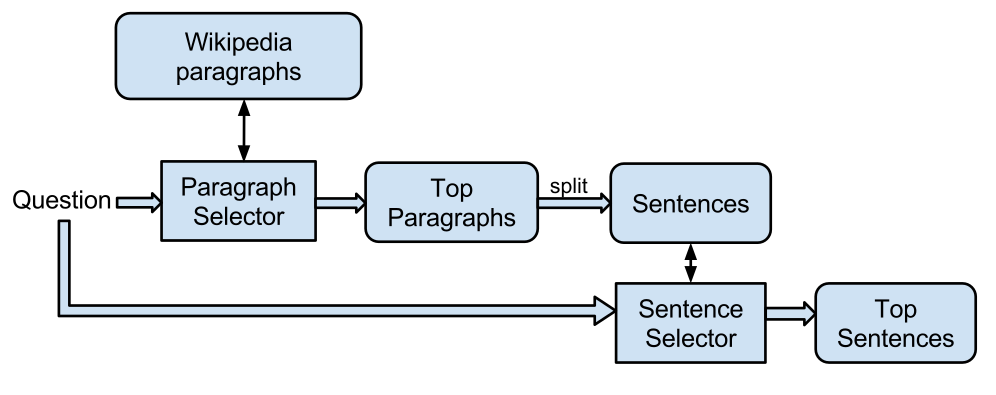
\includegraphics[width=\textwidth]{src/img/pipeline-lexical.png}
  \caption{The lexical filtering part of the pipeline}
  \label{fig:pipeline-lexical}
\end{figure}

In the case of the paragraph selector, the paragraphs are assigned a score solely based on the Lucene matching score. Based on this score, the first {\em N} paragraphs with the highest score are returned. $ N $ is a value that can be controlled at the initialization of the agent. This value may affect the accuracy and it is important that it $ N $ is chosen appropriately.

After the selection, the top paragraphs are split into sentences (using Stanford CoreNLP's "ssplit" annotator) and are added to the set that will be given to the sentence selector. The main difference of the two selectors is that the sentence selector scores the sentences not only based on the matching score between the query and a given sentence, but also takes into consideration the score of the paragraph that contains the respective sentence. The score is computed using the function in \autoref{eq:score}, where $ S $ is the score function in relation to a query, $ s $ is a given sentence, $ p $ is a paragraph (in which the sentence $ s $ must appear), $ \alpha_{p} $ is a weight signifying the importance of the paragraph for a given sentence, $ \alpha_{s} $ is the weight of the sentence (can be taken as $ 1 - \alpha_{p} $ ) and $ S_{Lucene} $ is the score given by Apache Lucene.

\begin{equation}
  S(s, q) = \alpha_{p} * S(p, q) + \alpha_{s} * S_{Lucene}(s, q)
  \label{eq:score}
\end{equation}

After the lexical pipeline returns the most likely sentences to answer the question, they are passed to the syntactic sieve. The role of the syntactical part of the pipeline is to re-score the sentences based on the possibility that they can answer the question. This syntactical filtering is done only considering the subject and predicate of the verb, therefore, if a sentence considered for selection has the same verb (or a synonym) with the verb representing the predicate in the question, then it is implied that the subject must match.

Having the question "When were you born?", addressed to John Lennon (the character the conversational agent was instantiated with), and two sentences, retrieved by the lexical pipeline, presented in \ref{eq:ans1} and \ref{eq:ans2}, we can apply the syntactic selection. It can be easily seen that the verb of the question is "born" and the subject is "you", which, in this case, refers to John Lennon. This means that the answers that have as a predicate the verb "to bear" must be linked to a subject that also refers to John Lennon, in this case. Using Stanford CoreNLP, the differentiation can be made.

\begin{equation}
  \text{\parbox{.85\textwidth}{Lennon was on tour when his first son, Julian, was born in April.}}
  \label{eq:ans1}
\end{equation}
\begin{equation}
  \text{\parbox{.85\textwidth}{Lennon was born in war-time England, on 9 October 1940 at Liverpool Maternity Hospital to Julia (née Stanley) and Alfred Lennon, a merchant seaman of Irish descent, who was away at the time of his son's birth.}}
  \label{eq:ans2}
\end{equation}

In this example, in the first sentence (\ref{eq:ans1}), the predicate "born" is obviously in relation with "first son", which is the subject and, therefore, must be excluded or, at least, have the score of the sentence decreased. On the other hand, the second statement (\ref{eq:ans2}) can be preserved in this syntactic analyzation step because the verb "born" is in relation with "Lennon" exactly like in the question.

\subsubsection{Question rephrasing}
\label{sub-sub-sec:rephrasing}

Because a phrase can be expressed in numerous ways by changing the order of the words and even the words (by replacing them with synonyms), the lexical form of a word in not enough to use it as a matching method between the question and the potential answers. To overcome that, the selectors in the pipeline that use the given question as input use methods of generating alternatives for that question.

Question rephrasing is done with the help of the synsets in WordNet. Using WordNet, for every word from the kernel question, a list of synonyms (including the initial word) is selected. The list is kept ordered as the JWI API returns it, indicating the importance (quantified by the {\em frequency count}) of the word. After this, all permutations of the synonyms are generated to get all the reformulations of the given query. The permutations are obtained using a simple implementation of the backtracking algorithm.


\ignore{
Answer sentence selection

To get the best results out of this approach, we need to follow a number of steps.
First, we need to remove unnecessary words, including stop words, the interrogative words (what, when, where, who, why and how) and irrelevant verbs (“to be”, “to have” and other similar verbs as described above) in order to remain only with meaningful words, i.e. the kernel of the question.
Second, we want to use the Stanford CoreNLP software to lemmatize the question (i.e. to convert every word to its appropriate canonical form) because, as described later on, the corpus used for a historical figure will be lemmatized too. This will help in the search step because words will more likely match if they are in their base form.
Third, we try to find alternative ways of expressing the input question and attempt to search for all this variants in the biographical text. We do this by trying different synonyms for the words in the question so that we can get more results, even if the initial question is formulated in such a way that it does not contain the exact words that might appear in the sentence representing the correct answer.
Next, the top paragraphs from the Wikipedia article are filtered based on the textual matching score between the question and the respective paragraph given by Apache Lucene [1], a text search tool. Then, we apply the same algorithm at the level of sentences instead of paragraphs. In short, to get the best answer the corpus is divided in separate paragraphs and a small set of paragraphs where the answer sentence might be part of are selected. Next, we attempt to find an even smaller set, made of sentences that are the best candidates to answer the question.
After we have a set of sentences that passed the lexical filtering, we want to eliminate those in which the subject of the sentence does not match the subject of the question. These mechanism is similar to maintaining the semantic relations as described in [5], and presented above in the Related Work section. To achieve that, we want to use Stanford CoreNLP, and in particular the Stanford Deterministic Co-reference Resolution System, to determine who is the subject of a given sentence.
After the syntactic filtering we are left only with the semantic filtering. This means we want to filter out all the sentences that do not have the type as the one expected by the question. For example, questions starting with “When” expect a answer sentence that contains a numerical value.
Finally, we choose the first sentence in order of the previously gathered relevance scores. Using the aforementioned approach we manage to answer more complex questions.
}
\section{Testing}
\label{sec:testing}

The testing of the conversational was done by hand by fetching a Wikipedia article of a random person and randomly selecting 10 to 20 sentences, attempting to formulate a question that could be answered by these sentences and then submitting the question to the conversational agent. If the conversational agent would return the selected sentence it means that it correctly answered the question. Of course, the questions can be formulated in a lot of ways, but the question rephrasing system in the implementation should take care of that.

In addition to these haphazardly selected sentences, the testing was also done with general questions like: "Where were you born?", "When did you die?", "Who was your husband/wife?" etc.
